%% !TEX program = xelatex
\documentclass[12pt,final]{novelette} % font size, twoside, twocolumn, draft-final, use extarticle for 8-20pt

\title{Diff Eq Final 2544}
\author{Kaka Cring}
\date{\today}

\begin{document}

\makeheading{ตัวอย่างข้อสอบ 2301312 สมการเชิงอนุพันธ์ ปรับปรุงจากข้อสอบไล่ภาคปลาย ปีการศึกษา 2544}

\subsubsection*{PART A}

\begin{question}
    \item {}
    จงหาผลเฉลยในรูปอนุกรมกำลังรอบจุด $x=0$ ของสมการ $2x^2y'' + x(2x+1)y' - y = 0$ โดยวิธีของโฟรเบนิอุส \qmark{12}

    % ----------------------------------------

    % ----------------------------------------

    \item {}
    จงหาค่าของ
    \begin{question}
        \item
        $\displaystyle \int_0^\infty e^{-x^4} \dd{x} \quad \text{(ให้ $t = x^4$)}$ \qmark{3}

        % ----------------------------------------
        \begin{align*}
            \int_0^\infty \frac14 e^{-t} t^{-3/4} \dd{t} & = \frac14 \mathcal{L}\left\{t^{-3/4}\right\}(1) \\
                                                         & = \boxed{\frac14 \Gamma\left(\frac14\right)}
        \end{align*}
        % ----------------------------------------

        \item
        $\displaystyle \int_{2\pi}^\infty e^{-4t} \sin 2t \cos 2t \dd{t}$ \qmark{4}

        % ----------------------------------------
        \begin{align*}
            \int_0^\infty \frac12 H(t-2\pi) e^{-4t} \sin 4t \dd{t} & = \frac12 \mathcal{L}\left\{H(t-2\pi) \sin 4t \right\}(4)                \\
                                                                   & = \frac14 e^{-2\pi \cdot 4} \mathcal{L}\left\{\sin(4t + 2\pi)\right\}(4) \\
                                                                   & = \boxed{\frac{e^{-8\pi}}{32}}
        \end{align*}
        % ----------------------------------------

    \end{question}

    \item {}
    จงเขียนสมการเชิงอนุพันธ์ที่มี $P_4(x)$ เป็นผลเฉลย พร้อมทั้งหา $P_4(x)$ \qmark{3}

    % ----------------------------------------
    \bigskip
    Legendre's differential equation of order $4$ is
    $$
        \boxed{(1-x^2)y'' - 2xy' + 20y = 0}
    $$

    Use Rodrigues' Formula
    \begin{align*}
        P_4(x) & = \frac{1}{2^n n!} \dv[n]{x} (x^2 - 1)^n \bigg|_{n=4}                                   \\
               & = \frac{1}{2^4 4!} \dv[4]{x} (x^2 - 1)^4                                                \\
               & = \frac{1}{2^4 4!} \dv[4]{x} (x^8 - 4x^6 + 6x^4)                                        \\
               & = \frac{1}{2^4 4!} (8\cdot7\cdot6\cdot5 x^4 - 4\cdot6\cdot5\cdot4\cdot3 x^2 + 6\cdot4!) \\
               & = \boxed{\frac{1}{8} (35x^4 - 30x^2 + 3)}
    \end{align*}
    % ----------------------------------------

    \item {}
    จงหาผลเฉลยของสมการ $\displaystyle xy'' + y' - \left(\frac1x - \frac x4\right)y = 0$ \qmark{8}

    % ----------------------------------------

    % ----------------------------------------

\end{question}

\subsubsection*{PART B}

\begin{question}[resume]
    \item {}
    จงเติมเฉพาะคำตอบลงในช่องว่างที่กำหนดให้โดยไม่ต้องแสดงวิธีทำ \qmark{5}
    \begin{multicols}{2}
        \begin{question}
            \everymath={\displaystyle}
            \item
            $\mathcal{L}\left\{\frac12\right\} = \boxed{\frac{1}{2s}}$

            \item
            $\mathcal{L}\left\{\sin 2t\right\} = \boxed{\frac{2}{s^2+4}}$

            \item
            $\mathcal{L}\left\{\cos 3t\right\} = \boxed{\frac{s}{s^2+9}}$

            \item
            $\mathcal{L}\left\{e^{-4t}\right\} = \boxed{\frac{1}{s+4}}$

            \item
            $\mathcal{L}\left\{t^2\right\} = \boxed{\frac{2}{s^3}}$

            \item
            $\mathcal{L}^{-1}\left\{\frac3s\right\} = \boxed{3}$

            \item
            $\mathcal{L}^{-1}\left\{\frac{s}{s^2+9}\right\} = \boxed{\cos 3t}$

            \item
            $\mathcal{L}^{-1}\left\{\frac{1}{s-5}\right\} = \boxed{e^{5t}}$

            \item
            $\mathcal{L}^{-1}\left\{\frac{1}{s^3}\right\} = \boxed{\frac{t^2}{2}}$

            \item
            $\mathcal{L}^{-1}\left\{\frac{1}{s^2+5}\right\} = \boxed{\frac{\sin(\sqrt5 t)}{\sqrt5}}$
        \end{question}
    \end{multicols}

    \item {}
    จงทำให้เป็นผลสำเร็จ \qmark{10}
    \begin{multicols}{2}
        \begin{question}
            \everymath={\displaystyle}
            \item
            $\int_0^\infty e^{(4-s)t} \dd{t} = \boxed{\frac{1}{s-4}}$

            \item
            $\int_0^\infty e^{-st} (t^2 - 2) \dd{t} = \boxed{\frac{2}{s^3} - \frac{2}{s}}$

            \item
            $\mathcal{L}\left\{4t^{3/2}\right\} = \boxed{\frac{3\sqrt\pi}{4s^{5/2}}}$

            \item
            $\mathcal{L}\left\{e^t \cos 2t\right\} = \boxed{\frac{s-1}{(s-1)^2+4}}$

            \item
            $\mathcal{L}\left\{t \sin 3t\right\} = \boxed{\frac{6s}{(s^2+9)^2}}$
        \end{question}
    \end{multicols}

    \item {}
    จงใช้ทฤษฎีบทสังวัตนาการหา $\displaystyle \mathcal{L}^{-1}\left\{\frac{s^2}{(s^2+1)^2}\right\}$ \qmark{5}

    % ----------------------------------------
    \bigskip
    By Convolution Theorem, $\mathcal{L}^{-1}\left\{F(s)G(s)\right\} = f(t)*g(t)$;
    \begin{align*}
        \mathcal{L}^{-1}\left\{\frac{s^2}{(s^2+1)^2}\right\} & = \mathcal{L}^{-1}\left\{\frac{s}{s^2+1}\frac{s}{s^2+1}\right\} \\
                                                             & = \cos t * \cos t                                               \\
                                                             & = \int_0^t \cos(u) \cos(u-t) \dd{u}                             \\
                                                             & = \frac12 \int_0^t \cos(2u - t) + \cos(t) \dd{u}                \\
                                                             & = \frac12 \left[\frac{\sin(2u - t)}{2} + u\cos t\right]_0^t     \\
                                                             & = \boxed{\frac12 (\sin t + t \cos t)}
    \end{align*}
    % ----------------------------------------

    \item {}
    จงใช้การแปลงลาปลาซหาผลเฉลยของสมการ $\displaystyle \dv{y}{t} + 2y + 2 \int_0^t y(t-x) \dd{x} = 2t; \quad y(0) = 0$ \qmark{7}

    % ----------------------------------------
    \bigskip
    Laplace transform both sides; $y(t) \xrightarrow{\mathcal{L}} Y(s)$
    \begin{align*}
        s Y(s) - y(0) + 2 Y(s) + 2 \mathcal{L}\left\{1*y(t)\right\} & = \frac2{s^2}          \\
        (s + 2) Y(s) + \frac2{s} Y(s)                               & = \frac2{s^2}          \\
        (s^2 + 2s + 2) Y(s)                                         & = \frac2s              \\
        Y(s)                                                        & = \frac2{s((s+1)^2+1)} \\
    \end{align*}

    \vspace{-2em}

    Use Convolution Theorem
    \begin{align*}
        y(t) & = 2\mathcal{L}^{-1}\left\{\frac1s\frac1{(s+1)^2+1}\right\} \\
             & = 2 \left[1 * (e^{-t} \sin t)\right]                       \\
             & = 2 \int_0^t e^{-u} \sin u \dd{u}                          \\
             & = \left[e^{-u} (-\cos u) + e^{-u} (- \sin u)\right]_0^t    \\
             & = \boxed{1 - e^{-t}(\sin t + \cos t)}
    \end{align*}
    % ----------------------------------------
\end{question}

\subsubsection*{PART C}

\begin{question}[resume]
    \item {}
    จงทำให้เป็นผลสำเร็จ \qmark{18}
    \begin{question}
        \everymath={\displaystyle}
        \item
        $\mathcal{L}\left\{\int_0^t e^x \cos 2x \dd{x}\right\} = \boxed{\frac1s \frac{s-1}{(s-1)^2 + 4}}$

        \item
        $\mathcal{L}\left\{\frac{e^t - e^{-2t}}{t}\right\}$
        \vspace*{-3.91em}
        \begin{flalign*}
            \phantom{\mathcal{L}\left\{\frac{e^t - e^{-2t}}{t}\right\}} & = \int_s^\infty \mathcal{L}\left\{e^t - e^{-2t}\right\}(r) \dd{r} & \\
                                                                        & = \int_s^\infty \frac{1}{r-1} - \frac{1}{r+2} \dd{r}                \\
                                                                        & = \lim_{a\to\infty} \left[\ln|r-1| - \ln|r+2|\right]_s^a            \\
                                                                        & = \boxed{\ln\frac{s-1}{s+2}}
        \end{flalign*}

        \item
        $\mathcal{L}^{-1}\left\{\frac{2}{s-3} + \frac{s}{9s^2+1}\right\} = \boxed{2e^{3t} + \frac{\cos t}{9}}$

        \item
        $\mathcal{L}^{-1}\left\{\frac{e^{-3s}}{s+1}\right\} = \boxed{H(t-3) e^{-(t-3)}}$

        \item
        $\mathcal{L}^{-1}\left\{\ln \frac{s-1}{s}\right\} = \boxed{\frac{e^t - 1}{t}}$

        \item
        $\mathcal{L}^{-1}\left\{\frac{s}{s^2+2s+10}\right\} =$
        \vspace*{-3.67em}
        \begin{flalign*}
            \phantom{\mathcal{L}^{-1}\left\{\frac{s}{s^2+2s+10}\right\}} & = \mathcal{L}^{-1}\left\{\frac{s}{(s+1)^2+9}\right\}                         & \\
                                                                         & = \mathcal{L}^{-1}\left\{\frac{s+1}{(s+1)^2+9} - \frac{1}{(s+1)^2+9}\right\}   \\
                                                                         & = \boxed{e^{-t}\left(\cos 3t - \frac13 \sin 3t\right)}
        \end{flalign*}
    \end{question}

    \item {}
    จงหาผลเฉลยของสมการ $\displaystyle y'' + y =
        \begin{cases}
            t,   & 0 < t < \pi \\
            \pi, & t > \pi
        \end{cases} ; \quad y(0) = 2, \quad y'(0) = 3$ \qmark{7}

    % ----------------------------------------
    \bigskip
    Rewrite into a heaviside function
    \begin{align*}
        y'' + y                          & = t - H(t-\pi)(t - \pi)
        \intertext{Laplace transform both sides; $y(t) \xrightarrow{\mathcal{L}} Y(s)$}
        s^2 Y(s) - s y(0) - y'(0) + Y(s) & = \frac{1}{s^2} - \frac{e^{-\pi s}}{s^2}                                                                                 \\
        (s^2 + 1) Y(s) - 2s - 3          & = \frac{1}{s^2} - \frac{e^{-\pi s}}{s^2}                                                                                 \\
        Y(s)                             & = \frac1{s^2+1}\left(\frac{1}{s^2} - \frac{e^{-\pi s}}{s^2} + 2s + 3\right)                                              \\
        y(t)                             & =  \mathcal{L}^{-1}\left\{\frac1{s^2+1}\left(\frac{1}{s^2} - \frac{e^{-\pi s}}{s^2}\right)\right\} + 2 \cos t + 3 \sin t \\
    \end{align*}

    \vspace{-2em}

    The first part (use Convolution Theorem)
    \begin{align*}
        \mathcal{L}^{-1}\left\{\frac{1}{s^2+1}\frac{1}{s^2}\right\} & = \sin t * t                                      \\
                                                                    & = \int_0^t \sin u (t - u) \dd{u}                  \\
                                                                    & = \left[- t \cos u + u \cos u - \sin u\right]_0^t \\
                                                                    & = - \sin t + t
    \end{align*}

    The second part (use $\mathcal{L}^{-1}\left\{e^{-as}F(s)\right\} = f(t-a) H(t-a)$)
    \begin{align*}
        \mathcal{L}^{-1}\left\{e^{-\pi s}\frac{1}{s^2+1}\frac{1}{s^2}\right\} & = H(t - \pi) (- \sin(t - \pi) + t - \pi) \\
                                                                              & = H(t - \pi) (\sin t + t - \pi)
    \end{align*}

    The final result
    \begin{align*}
        y(t)          & = - \sin t + t - H(t - \pi)(\sin t + t - \pi) + 2 \cos t + 3 \sin t \\
                      & = t + 2 \cos t + 2 \sin t - H(t - \pi)(\sin t + t - \pi)            \\
        \Aboxed{ y(t) & =
        {
        \begin{cases}
            t + 2 \cos t + 2 \sin t, & \text{if}\ 0 < t < \pi \\
            \pi + 2 \cos t + \sin t, & \text{if}\ t > \pi
        \end{cases}
        }
        }
    \end{align*}
    % ----------------------------------------

    \item {}
    จงหาผลเฉลยของระบบสมการเชิงอนุพันธ์\\[.5em]
    \hspace*{.5cm}$
        \left\{\begin{aligned}
            (D-1)x + y  & = 2 \sin t         \\[.2em]
            -x + (D+1)y & = 4\cos t - \sin t
        \end{aligned}\right.
    $ \quad เมื่อ $x(0) = 2, \quad y(0) = 5$ \qmark{8}

    % ----------------------------------------
    \vspace*{-1em}
    \begin{align*}
        \intertext{Find determinant of differential operators}
        P(D)   & =
        \begin{vmatrix}
            D - 1 & 1     \\
            -1    & D + 1
        \end{vmatrix} = D^2                                         \\
        \intertext{Find $x(t)$}
        P(D) x & =
        \begin{vmatrix}
            2 \sin t          & 1   \\
            4 \cos t - \sin t & D+1
        \end{vmatrix}                                     \\
        D^2 x  & = (D+1) 2 \sin t - 4 \cos t + \sin t               \\
        D^2 x  & = (3 \sin t - 2 \cos t)                            \\
        x      & = c_1 + c_2 t + \frac{1}{D^2}(3 \sin t - 2 \cos t) \\
        x      & = c_1 + c_2 t - 3 \sin t + 2 \cos t                \\
        \intertext{Find $y(t)$}
        P(D) y & =
        \begin{vmatrix}
            D - 1 & 2 \sin t          \\
            -1    & 4 \cos t - \sin t
        \end{vmatrix}                                   \\
        D^2 y  & = (D-1)(4 \cos t - \sin t) + 2 \sin t              \\
        D^2 y  & = - \sin t - 5 \cos t                              \\
        y      & = c_3 + c_4 t + \frac{1}{D^2}(- \sin t - 5 \cos t) \\
        y      & = c_3 + c_4 t + \sin t + 5 \cos t
    \end{align*}

    Substitute $x(t)$ and $y(t)$ into equation
    \begin{align*}
        (D-1) x + y     & = 2 \sin t \\
        \begin{aligned}
            (D-1) (c_1 + c_2 t - 3 \sin t + 2 \cos t) \hspace*{2.5em} \\
            + c_3 + c_4 t + \sin t + 5 \cos t
        \end{aligned}
                        & = 2 \sin t \\
        \begin{aligned}
            c_2 - \cancel{3 \cos t} - 2 \sin t \hspace*{8.5em}             \\
            - \,c_1 - c_2 t + 3 \sin t - \cancel{2 \cos t} \hspace*{2.5em} \\
            + \,c_3 + c_4 t + \sin t + \cancel{5 \cos t}
        \end{aligned}
                        & = 2 \sin t \\
        - c_2 +c_4      & = 0        \\
        c_2 - c_1 + c_3 & = 0        \\
    \end{align*}

    \vspace{-1em}

    Rewrite with 2 constants
    \begin{align*}
        x & = c_1 + c_2 t - 3 \sin t + 2 \cos t       \\
        y & = (c_1 - c_2) + c_2 t + \sin t + 5 \cos t
    \end{align*}

    Check with initial conditions
    \begin{center}
        $x(0) = 2 \implies c_1 + 2 = 2 \implies c_1 = 0$ \\[.5em]
        $y(0) = 5 \implies -c_2 + 5 = 5 \implies c_2 = 0$
    \end{center}

    The final results are
    \medskip
    \[
        \boxed{
            \begin{aligned}
                x & = -3 \sin t + 2 \cos t \\
                y & = \sin t + 5 \cos t
            \end{aligned}
        }
    \]
    % ----------------------------------------

\end{question}

\subsubsection*{PART D}

\begin{question}[resume]
    \item {}
    กำหนดฟังก์ชัน
    $f(x) = \begin{cases}
            0,       & -\pi < x < 0 \\
            \pi - x, & 0 < x < \pi
        \end{cases}$ และ $f(x + 2\pi) = f(x)$
    \begin{question}
        \item
        จงเขียนกราฟของฟังก์ชัน $f(x)$ บนช่วง $(-3\pi, 3\pi)$

        % ----------------------------------------
        \medskip
        \begin{center}
            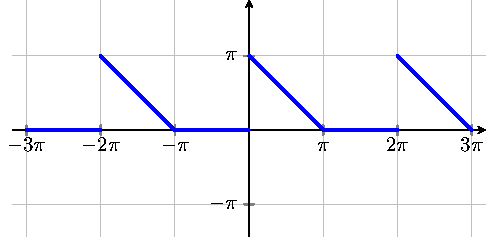
\includegraphics{images/graph.pdf}
        \end{center}
        % ----------------------------------------

        \item
        จงหาอนุกรมฟูเรียร์ของฟังก์ชัน $f(x)$

        % ----------------------------------------

        % ----------------------------------------

        \item
        จงหาผลบวกของ $\displaystyle \sum_{n=1}^{\infty} \frac{1}{(2n - 1)^2}$ \qmark{10}

        % ----------------------------------------

        % ----------------------------------------
    \end{question}

    \item {}
    เส้นลวดมีความยืดหยุ่นเส้นหนึ่งยาว $\pi$ หน่วย ปลายทั้งสองถูกยึดติดแน่นที่จุด $x = 0$ และ $x = \pi$ \\
    เส้นลวดนี้ถูกทำให้เป็นเส้นโค้ง $u(x, 0) = x(\pi - x)$ แล้วปล่อยให้เกิดการสั่นด้วยความเร็ว $u_t(x, 0) = 3$ \\
    จงเขียนปัญหาค่าเริ่มต้นและค่าขอบของโจทย์นี้โดยไม่ต้องหาผลเฉลย (กำหนดให้ $c^2 = 1$) \qmark{3}

    % ----------------------------------------

    % ----------------------------------------

    \item {}
    จงแสดงวิธีหาผลเฉลยของปัญหาค่าเริ่มต้นและค่าขอบซึ่งถูกควบคุมด้วยสมการความร้อนใน $1$ มิติ
    $$
        \pdv{u}{t} = c^2 \pdv[2]{u}{x}, \quad 0 < x < L, \quad t > 0
    $$
    ภายใต้เงื่อนไขขอบ \quad $u(0, t) = 0, \quad u(L, t) = 0, \quad t \geq 0$ \\
    และเงื่อนไขเริ่มต้น \quad $u(x, 0) = f(x), \quad 0 < x < L$ \qmark{12}

    % ----------------------------------------

    % ----------------------------------------

    \item {}
    จงหาผลเฉลยของปัญหาในข้อ 14 เมื่อกำหนดให้ $c^2 = 9, L = 4, f(x) = x + 12$ \qmark{5}

    % ----------------------------------------

    % ----------------------------------------
\end{question}

\subsubsection*{PART E}

\begin{question}[resume]
    \item {}
    จงหาผลเฉลยในรูปอนุกรมกำลังรอบจุดสามัญ $x = 0$ ของสมการ $y'' - xy' - y = 0$ \\
    (เขียนผลเฉลยให้เห็นอย่างน้อยถึงพจน์ $x^5$) \qmark{10}

    % ----------------------------------------
    \bigskip
    (From midterm q.13) The solution is
    $$
        \boxed{y = c_1\left(1 + \frac{x^2}{2} + \frac{x^4}{8} + \cdots\right) + c_2\left(x + \frac{x^3}{3} + \frac{x^5}{15} + \cdots\right)}
    $$
    % ----------------------------------------

    \item {}
    ลวดสปริงเส้นหนึ่งถูกยึดปลายบนติดกับเพดาน
    เมื่อนำวัตถุหนัก $6$ ปอนด์ มาผูกติดไว้ที่ปลายล่างของลวดปริงจะทำให้ลวดสปริงยืดออก $6$ นิ้ว
    ถ้าดึงวัตถุนี้ลงมาต่ำกว่าตำแหน่งสมดุล $4$ นิ้ว แล้วปล่อยด้วยการผลักวัตถุขึ้นด้วยความเร็ว $\frac83$ ฟุต/วินาที \\
    จงหาสมการของการเคลื่อนที่ของวัตถุ พร้อมทั้งบอกค่าแอมพลิจูด และมุมทิ้งช่วง \qmark{10}

    % ----------------------------------------
    \bigskip
    (From midterm q.3) The motion equation is
    $$
        \boxed{x(t) = \frac{\sqrt2}{3}\sin\left(8t+\frac{3\pi}{4}\right)\,\si{ft}}
    $$
    Amplitude is $\boxed{\frac{\sqrt2}3\,\si{ft}}$ and angle of departure is $\boxed{\frac{3\pi}{4}\,\si{rad}}$.
    % ----------------------------------------

    \item {}
    สำหรับปัญหาการเคลื่อนที่ของวัตถุที่ผูกติดกับปลายลวดสปริงปัญหาหนึ่ง
    ถ้าเราทราบว่าสมการของการเคลื่อนที่ของวัตถุคือ
    $$
        x(t) = \frac13 \sin\left(\pi t - \frac\pi4\right)
    $$
    \begin{question}
        \item
        จงหา แอมพลิจูด คาบ และความถี่ของการเคลื่อนที่ \qmark{1.5}

        % ----------------------------------------
        \bigskip
        (From midterm q.4) Amplitude is $\boxed{\frac13}$. Period is $\boxed{2}$. Frequency is $\boxed{\frac12}$.
        % ----------------------------------------

        \item
        จงหาตำแหน่ง ความเร็ว ความเร่งของการเคลื่อนที่ เมื่อเวลา $1$ วินาที หลังจากปล่อยให้วัตถุเกิดการเคลื่อนที่
        พร้อมทั้งอธิบายลักษณะของการเคลื่อนที่ของวัตถุ ณ ขณะนั้น \qmark{3.5}

        % ----------------------------------------
        \phantom{}
        \vspace*{-1em}
        \begin{align*}
            x(1)   & = \frac13 \sin\left(\pi - \frac\pi4\right)   \\
                   & = \boxed{\frac1{3\sqrt2}}                    \\
            x'(1)  & = \frac\pi3 \cos\left(\pi - \frac\pi4\right) \\
                   & = \boxed{\frac{\pi}{3\sqrt2}}                \\
            x''(1) & = \boxed{-\frac{\pi^2}{3\sqrt2}}
        \end{align*}

        The object is travelling in $+x$ direction and is getting accelerated into $-x$ direction.
        % ----------------------------------------
    \end{question}

    \item {}
    จงหาประจุไฟฟ้า $q(t)$ บนตัวเก็บประจุในวงจรไฟฟ้าแบบอนุกรม $RLC$ ที่เวลา $t = 0.01$ วินาที \\
    เมื่อ $L = 0.05$ เฮนรี, $C = 0.01$ ฟารัด, $E(t) = 0$ โวลต์, $q(0) = 5$ คูลอมบ์ และ $i(0) = 0$ แอมแปร์
    และจงพิจารณาหาเวลาที่ประจุไฟฟ้าบนตัวเก็บประจุเป็นศูนย์ครั้งแรก \qmark{10}

    % ----------------------------------------

    % ----------------------------------------
\end{question}

\end{document}